\section{Case Studies} \label{sec:casestudies}

% Intuitively, adding structure information to a random generator should provide
% better results when verifying a system using random testing.
%
% For instance, by generating values that are no only syntactically but also
% semantically meaningful we would expect to reach deeper stages of our program
% pipeline other than merely input parsing/validation.
%
This section describes two case studies showing that considering additional
structural information when deriving generators can consistently produce better
testing results in terms of code coverage.
%
Instead of restricting our scope to Haskell, in this work we follow a broader
evaluation approach taken previously to compare state-of-the-art techniques to
derive random data generators based on ADT definitions
\cite{grieco2017,DBLP:conf/haskell/MistaRH18}.
%

We evaluate how including additional structural information when generating a
set of random test cases (often referred as a \emph{corpus}) affects the code
coverage obtained when testing a given target program.
%
For that, we considered two external programs which expect highly structured
inputs, namely \emph{GNU
  CLISP} \footnote{\href{https://www.gnu.org/software/gcl/}{https://www.gnu.org/software/gcl/}}---the
GNU Common Lisp compiler, and \emph{HTML Tidy}
\footnote{\href{http://www.html-tidy.org}{http://www.html-tidy.org}}---a well
known HTML refactoring and correction utility.
%
We remark that these applications are not written in Haskell.
%
However, there exist Haskell libraries defining ADTs encoding their input
structure, i.e., Lisp and HTML values respectively. These libraries are:
\emph{hs-zuramaru}\footnote{\href{http://hackage.haskell.org/package/zuramaru}{http://hackage.haskell.org/package/zuramaru}},
implementing an embedded Lisp interpreter for a small subset of this programming
language, and
\emph{html}\footnote{\href{http://hackage.haskell.org/package/html}{http://hackage.haskell.org/package/html}},
defining a combinator library for constructing HTML values.
%
These libraries also come with serialization functions to map Haskell values
into corresponding test case files.


We firstly compiled instrumented versions of the target programs in a way that
they also return the execution path followed in the source code every time we
run them with a given input test case.
%
This let us distinguish the amount of different execution paths that a randomly
generated corpus can trigger.
%
We then used the ADTs defined on the chosen libraries to derive random
generators using \dragen and \dragenp, including structural information
extracted from the library's codebase in the case of the latter.
%
Then, we proceeded to evaluate the code coverage triggered by independent,
randomly generated corpora of different sizes varying from 100 to 1000 test
cases each.
%
In order to remove any external bias, we derived generators optimized to follow
\emph{a uniform distribution of constructors (and pattern matchings or function
  calls in the case \dragenp), and carefully adjusted their generation sizes to
  match the average test case size in bytes}.
%
This way, any noticeable difference in the code coverage can be attributed to
the presence (or lack thereof) structural information when generating the test
cases.
%
Additionally, to achieve statistical significance we repeated each experiment 30
times with independently generated sets of random test cases.

\begin{figure*}[t]
  \vspace{-10pt}%
  \centering
  \pgfplotsset{scaled y ticks=false}
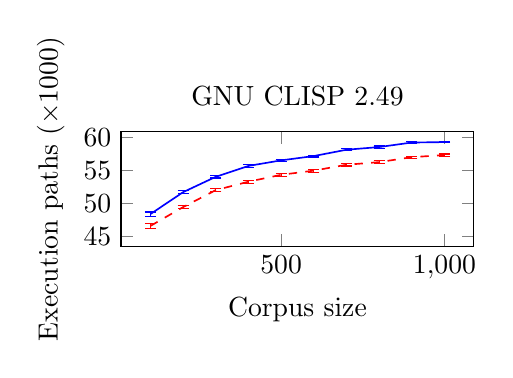
\begin{tikzpicture}
  \begin{axis}[
    title={GNU CLISP 2.49},
    height=0.25\textwidth,
    width=0.5\textwidth,
    xlabel={Corpus size},
    ylabel={Execution paths ($\times 1000$)},
    % y tick label style={rotate=45,anchor=east},
    % ymajorgrids=true,
    legend pos=south east,
    legend cell align={left},
    % xmin=100, xmax=1000,
    ymin=45, %ymax=23000,
    enlarge x limits=0.1,
    enlarge y limits=0.1
    ]
    \addplot+[blue][semithick, mark=none,
    error bars/.cd, y dir=both, y explicit]
    coordinates {
      (100,  48.39887) +- (0.0, 0.3148367)
      (200,  51.71763) +- (0.0, 0.1864931)
      (300,  54.04380) +- (0.0, 0.1782321)
      (400,  55.69140) +- (0.0, 0.1910262)
      (500,  56.53007) +- (0.0, 0.1775220)
      (600,  57.18347) +- (0.0, 0.1468032)
      (700,  58.14023) +- (0.0, 0.1508515)
      (800,  58.54617) +- (0.0, 0.1587068)
      (900,  59.23067) +- (0.0, 0.1255331)
      (1000, 59.29573) +- (0.0, 0.1014993)
    };
    % \addlegendentry{\dragenp};
    % \addplot+[blue][semithick, mark=none,
    % error bars/.cd, y dir=both, y explicit]
    % coordinates {
    %   (100,  12805.40) +- (0.0, 234.61546)
    %   (200,  15382.40) +- (0.0, 172.25118)
    %   (300,  16984.87) +- (0.0, 106.89291)
    %   (400,  17695.77) +- (0.0, 157.54098)
    %   (500,  18670.37) +- (0.0, 138.47555)
    %   (600,  19197.10) +- (0.0, 137.48348)
    %   (700,  19934.90) +- (0.0, 97.24403 )
    %   (800,  20430.27) +- (0.0, 129.08726)
    %   (900,  20775.97) +- (0.0, 136.66240)
    %   (1000, 21264.20) +- (0.0, 102.07806)
    % };
    % \addlegendentry{\dragenp};
    \addplot+[red][semithick, dashed, mark=none,
    error bars/.cd, y dir=both, y explicit,
    error bar style={solid}
    ]
    coordinates {
      (100,  46.60783) +- (0.0, 0.3282654)
      (200,  49.45887) +- (0.0, 0.2526707)
      (300,  52.02820) +- (0.0, 0.2725756)
      (400,  53.30213) +- (0.0, 0.2362873)
      (500,  54.34667) +- (0.0, 0.2026468)
      (600,  54.97770) +- (0.0, 0.2171262)
      (700,  55.86617) +- (0.0, 0.1812106)
      (800,  56.26630) +- (0.0, 0.1827455)
      (900,  57.01167) +- (0.0, 0.1654614)
      (1000, 57.33917) +- (0.0, 0.1598649)
    };
    % \addlegendentry{\dragen};
  \end{axis}
\end{tikzpicture}

  \hspace{5pt}%
  \pgfplotsset{scaled y ticks=false}
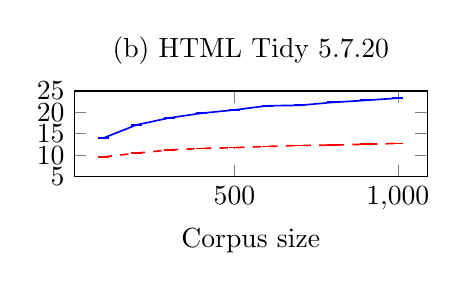
\begin{tikzpicture}
  \begin{axis}[
    title={(b) HTML Tidy 5.7.20},
    height=0.22\textwidth,
    width=0.5\textwidth,
    xlabel={Corpus size},
    % ylabel={Different execution paths (thousands)},
    % y tick label style={rotate=45,anchor=east},
    % ymajorgrids=true,
    legend pos=south east,
    legend cell align={left},
    % xmin=100, xmax=1000,
    ymin=5, ymax=25,
    enlarge x limits=0.1
    % enlarge y limits=0.1
    ]
    \addplot+[blue][semithick, mark=none,
    error bars/.cd, y dir=both, y explicit]
    coordinates {
      (100,  14.01417) +- (0.0, 0.14883523)
      (200,  17.05810) +- (0.0, 0.13506726)
      (300,  18.68763) +- (0.0, 0.11803936)
      (400,  19.80227) +- (0.0, 0.15292292)
      (500,  20.55840) +- (0.0, 0.13536179)
      (600,  21.53490) +- (0.0, 0.10085658)
      (700,  21.63750) +- (0.0, 0.10470160)
      (800,  22.32833) +- (0.0, 0.11168286)
      (900,  22.78813) +- (0.0, 0.10231978)
      (1000, 23.32330) +- (0.0, 0.09762431)
    };
    \label{exp:dragenp}
    % \addlegendentry{\dragenp};
    % \addplot+[blue][semithick, mark=none,
    % error bars/.cd, y dir=both, y explicit]
    % coordinates {
    %   (100,  12805.40) +- (0.0, 234.61546)
    %   (200,  15382.40) +- (0.0, 172.25118)
    %   (300,  16984.87) +- (0.0, 106.89291)
    %   (400,  17695.77) +- (0.0, 157.54098)
    %   (500,  18670.37) +- (0.0, 138.47555)
    %   (600,  19197.10) +- (0.0, 137.48348)
    %   (700,  19934.90) +- (0.0, 97.24403 )
    %   (800,  20430.27) +- (0.0, 129.08726)
    %   (900,  20775.97) +- (0.0, 136.66240)
    %   (1000, 21264.20) +- (0.0, 102.07806)
    % };
    % \addlegendentry{\dragenp};
    \addplot+[red][semithick, dashed, mark=none,
    error bars/.cd, y dir=both, y explicit,
    error bar style={solid}
    ]
    coordinates {
      (100,  09.574067) +- (0.0, 0.05736926)
      (200,  10.451433) +- (0.0, 0.04399278)
      (300,  11.195367) +- (0.0, 0.03931592)
      (400,  11.556767) +- (0.0, 0.04036912)
      (500,  11.738333) +- (0.0, 0.04965803)
      (600,  12.028333) +- (0.0, 0.04250789)
      (700,  12.257100) +- (0.0, 0.03936573)
      (800,  12.334567) +- (0.0, 0.04082921)
      (900,  12.536733) +- (0.0, 0.04470660)
      (1000, 12.731967) +- (0.0, 0.04069840)
    };
    \label{exp:dragen}
    % \addlegendentry{\dragen};
  \end{axis}
\end{tikzpicture}
  \caption{Path coverage comparison between \dragen (\ref{exp:dragen}) and
    \dragenp (\ref{exp:dragenp}). }
  \label{fig:coverage}
  \vspace{-12pt}%
\end{figure*}
%
Figure \ref{fig:coverage} illustrates the mean number of different execution
paths triggered for different combinations of corpus size and derivation tool,
including error bars indicating the standard error of the mean on each case.
%
We proceed to describe each case study and our findings in detail as follows.

\subsection{Branching on input data}

In this first case study we wanted to evaluate the observed code coverage
differences when considering structural information present on functions pattern
matchings.


Our chosen library encodes Lisp S-expressions essentially as lists of symbols,
represented as plain strings; and literal values like booleans or integers.
%
In order to interpret Lisp programs, this unified representation of data and
code requires this library to pattern match against common patterns like
let-bindings, if-then-else expressions and arithmetic operators among others.
%
In particular, each one of these patterns match a against special symbol of the
Lisp syntax like |"let"|, |"if"| or |"+"|; and their corresponding
sub-expressions.
%
We extracted this structural information and included it into the generation
specification of our random Lisp values---which were generated by randomly
picking from a total of 6 data constructors and 8 different pattern matchings.
%
By doing this, we obtained a code coverage improvement of approximately $4\%$
using \dragenp with respect to the one obtained with \dragen (see Figure
\ref{fig:coverage} (a)).
%
While it seems an small improvement, we argue that an improvement of $4\%$ is
not negligible considering (a) the little effort that took us to specify the
pattern matchings and (b) that we are testing a full-fledged compiler.
%it is worth noticing that we are generating
%highly structured inputs, i.e., Lisp programs.
%
%When testing interpreters,
%\todo[inline, author=AM]{Shall we say anything justifing this little
%  improvement?}

\subsection{Abstract interfaces}


For our second case study, we wanted to evaluate how including structural
information coming from abstract interfaces when generating random HTML values
might improve the testing performance.


The library we used for this purpose represents HTML values very much in the
same way as we exemplify in Section \ref{sec:randomtesting}, i.e., defining a
small set of general constructions representing plain text and tags---although
this library also supports HTML tag attributes as well.
%
Then, this representation is extended with a large abstract interface consisting
of combinators representing common HTML tags and tag attributes---equivalent to
the combinators |div|, |bold| and |hr| illustrated in Section \ref{sec:sources}.


In this case study we included the structural information present on the abstract
interface of this library into the generation specification of random HTML
values, resulting in a generation process that randomly picked among 4 data
constructors and 163 abstract functions.
%
With this large amount of additional structural information, we observed an
increase of up to $83\%$ in the code coverage obtained with \dragenp with
respect to the one observed with \dragen (see Figure \ref{fig:coverage} (b)).
%
A manual inspection of the corpora generated with each tool revealed us that, in
general terms, the test cases generated with \dragen rarely represent
syntactically correct HTML values, consisting to a large extent of random
strings within and between HTML tag delimiters (|"<"|, |">"| and |"/>"|).
%
On the other hand, test cases generated with \dragenp encode much more
interesting structural information, being mostly syntactically correct.
%
We found that, in many cases, the test cases generated with \dragenp were
parsed, analyzed and reported as valid HTML values by the target application.


With these results we are confident that including the structural information
present on the user codebase improves the overall testing performance.
%
%% Space reasons
%We consider that our approach is particularly useful when the data types
%encoding the shape of our data are vague or not sufficiently structured to be
%used to derive powerful random generators with the common derivation techniques
%based only on ADT definitions.
